\chapter{柱、锥、台、球}

\section{柱、锥、台、球的定义及性质}
本节将研究由点、直线、平面等元素构成的几何体,常
见的几何体有柱、锥、台、球。

\subsection{柱}

柱面是经常遇到的物体的表面形状。建筑物的
棱柱、圆柱的侧面都是柱面,这些侧面可以看作是由一条直
线运动所产生的。

\begin{blk}{定义}
    一条直线$\ell$在空间作平行于固定方向的运动,但
总和任一固定的曲线$C$相交,所产生的曲面叫做柱面、移动
的直线$\ell$所在的每个位置叫做柱面的母线,而在移动中始终
和母线相交的曲线$C$叫做柱面的准线。
\end{blk}

下面,我们考虑几种简单情况
\begin{enumerate}
\item 准线是一条直线,这时的柱面是一个平面(见图
2.1)。
\item 准线是一个平面多边形,这时的柱面叫做棱柱面
(见图2.2)。
\item 准线是一个圆,这时的柱面叫做圆柱面(图2.3)。
\end{enumerate}

\begin{figure}[htp]\centering
    \begin{minipage}[t]{0.3\textwidth}
    \centering
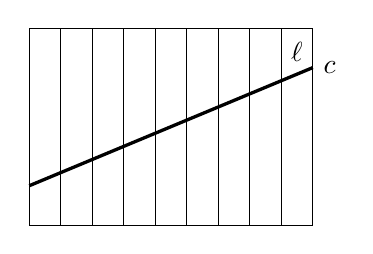
\begin{tikzpicture}[>=latex, scale=1]
\draw(0,0) rectangle (3.6,2.5);
\foreach \x in {.4,.8,1.2,...,2.8,3.2}
{
    \draw(\x,0)--(\x,2.5);
}
\draw[very thick](0,.5)--(3.6,2)node[right]{$c$};
\node at (3.2,2.2)[right]{$\ell$};
    \end{tikzpicture}
    \caption{}
    \end{minipage}
    \begin{minipage}[t]{0.3\textwidth}
    \centering
    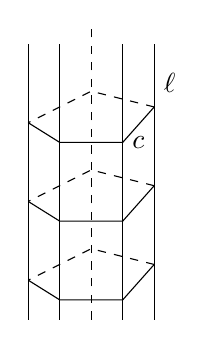
\begin{tikzpicture}[>=latex, scale=1]
\foreach \x in {0,.4,1.2,1.6}
{
    \draw(\x,0)--(\x, 3.5);
}
\draw[dashed](.8,0)--(.8, 3.7);
\foreach \x in {0,1,2}
{
    \draw(0,.5+\x)--(.4,.25+\x)--(1.2,.25+\x)--(1.6,.7+\x);
    \draw[dashed](1.6,.7+\x)--(.8,.9+\x)--(0,.5+\x);
}
\node at (1.6,3)[right]{$\ell$};
\node at (1.2,2.25)[right]{$c$};
    \end{tikzpicture}
    \caption{}
    \end{minipage}
        \begin{minipage}[t]{0.3\textwidth}
    \centering
    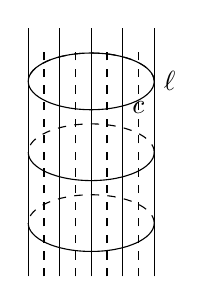
\begin{tikzpicture}[>=latex, yscale=.45]
\foreach \x in {0,.4,.8,1.2,1.6}
{
    \draw(\x,0)--(\x, 7);
}
\foreach \x in {.4,.8,1.2,1.6}
{
    \draw[dashed](\x-.2,0)--(\x-.2, 6.5);
}
\foreach \x in {1,2,3}
{
   \draw[dashed](1.6,-.5+\x*2) arc (0:180:.8);
   \draw (1.6,-.5+\x*2) arc (0:-180:.8);
}
\draw (1.6,-.5+3*2) arc (0:180:.8);
\node at (1.6,5.5)[right]{$\ell$};
\node at (1.6,5.2)[below left]{$c$};
    \end{tikzpicture}
    \caption{}
    \end{minipage}
    \end{figure}


以后我们只研究母线和该圆所在的平面垂直的圆柱面,
这种圆柱面叫\textbf{直圆柱面}。

\begin{blk}{定理}
    若平行平面与柱面的母线相交,则交线所成的图
形全等。
\end{blk}

\begin{proof}
    设平行平面$\alpha_1$和$\alpha_2$与柱面的母线相交,$\ell$是柱面上
任一条母线。令$P_1=\alpha_1\cap \ell$, $P_2=\alpha_2\cap\ell$, 我们称$P_1$和$P_2$是对
应点。显然$P_1$对应于$P_2$, $P_2$也对应于$P_1$, 并且不同位置的
两点$P_1$、$P'_1$对应于不同位置的两点$P_2$、$P_2'$(图2.4).

\begin{figure}[htp]
    \centering
    \includegraphics[scale=.7]{fig/2-4.png}
    \caption{}
\end{figure}


于是在平行平面与柱面所截出的两条截线上的点与点之间建立了一一对应关系。

设在两条截线上有任意三对对应
点:$A_1$对应于$A_2$, $B_1$对应于$B_2$, $C_1$对
应于$C_2$, 因为$A_1A_2,B_1B_2,C_1C_2$都
是夹在平行平面$\alpha_1$和$\alpha_2$之间柱面的母
线的一部分,故
\[A_1A_2\mathop{=}^{\parallel} B_1B_2\mathop{=}^{\parallel}C_1C_2\]
从而四边形$A_1A_2B_2B_1$和四边形$B_1B_2C_2C_1$都是平行四边形,
它们的对边相等,所以,$A_1B_1=A_2B_2$, $B_1C_1=B_2C_2$. 又因
为$\angle A_1B_1C_1$与$\angle A_2B_2C_2$的两边平行且同向,所以
$\angle A_1B_1C_1=\angle A_2B_2C_2$。

这样,平行平面和柱面的母线相交,交出的图形总能重
合,因此它们全等。
\end{proof}


\begin{blk}{定义} 
    由封闭的柱面和两个与母线都相交的平行平面所
围成的几何体叫做柱体。

柱体的柱面夹在平行平面之间的部分叫做柱体的\textbf{侧面},
两个平行平面与柱体的相交部分叫做柱体的\textbf{底面}。
    
\end{blk}

现在,我们来研究几个特殊的柱体。

\begin{blk}{定义} 
    如果一个柱体的侧面是棱柱面,那么这个柱体叫
做棱柱。如果一个柱体的侧面是圆柱面,那么这个柱体叫圆
柱体。    
\end{blk}

显然,由这个定义可以得到以下推论:
\begin{enumerate}
\item 棱柱的两个底面是对应边互相平行的全等多边
形。

全等多边形的顶点叫做柱棱的顶点。以全等多边形对应
顶点为端点的线段称为棱柱的侧棱,相邻两侧棱及其所夹的
两底全等多边形的两条对应边所组成的四边形称为棱柱的侧
面。显然,
\item 棱柱的各侧面全是平行四边形。
\item 棱柱的各侧棱平行且相等。
\end{enumerate}


\begin{blk}{定义}
    棱柱按底面是三角形,四边形……分别叫做三棱
柱、四棱柱……

如果棱柱的侧棱垂直于底面,那么这个棱柱叫做直棱
柱,否则叫做斜棱柱。

如果棱柱是直棱柱,并且其底面是正多边形,那么这棱
柱就叫做正棱柱。在正棱柱中,各侧面都是全等的矩形。
\end{blk}
 
\begin{blk}
    {定义}棱柱上不在同一个底面上也不在同一个侧面上的
两个顶点所连结的线段叫做棱柱的对角线;过不在同一个
侧面的两条侧棱作一个平面,这平面截棱柱所得的截面叫做
棱柱的对角面。两底面之间的距离叫做棱柱的高。
\end{blk}

\begin{figure}[htp]
    \centering
    \includegraphics[scale=.7]{fig/2-5.png}
    \caption{}
\end{figure}

图2.5是五棱柱,五边形$ABCDE$和$A'B'C'D'E'$是它
的两个底面,$ABB'A'$、$BCC'B'$等是它的侧面,$AA'$、$BB'$
等是它的侧棱,$HH'$的长是它的高。$A'C$是它的一条对角
线。

棱柱的表示法是写出两个底面各顶点
的字母,中间用一条短横线隔开,如图
2.5的五棱柱就表示作棱柱$ABCDE$-$A'
B'C'D'E'$. 也有用棱柱一条对角线的两
个端点表示棱柱的,如图2.5可表示作五
棱柱$A'C$. 

\begin{blk}{定义} 
    底面是平行四边形的四棱柱叫
    做平行六面体。其中侧棱和底面斜交的叫
    斜平行六面体,侧棱和底垂直的叫直平行六面体。底面是
    矩形的直平行六面体叫做长方体。交于一个顶点的三条棱的
    长相等的长方体叫做正方体,也叫立方体。(图2.6)
\end{blk}

\begin{figure}[htp]
    \centering
\begin{tikzpicture}
\begin{scope}
\tkzDefPoints{0/0/A, 1/0/B, 1.5/.5/C, .5/.5/D}
\tkzDefPoint(.25,2.2){A_1}
\tkzDefPointsBy[translation=from A to A_1](B,C,D){B_1,C_1,D_1}
\tkzDrawPolygon(A_1,B_1,C_1,D_1)
\draw(A)--(B)--(C);
\draw[dashed](A)--(D)--(C);
\draw[dashed](D_1)--(D);
\draw(A_1)--(A);\draw(B_1)--(B);\draw(C_1)--(C);
\node at (.5,-.5){斜平行六面体};
\end{scope}

\begin{scope}[xshift=3cm]
    \tkzDefPoints{0/0/A, .65/-.15/B, 2/0/C, 1.35/.15/D}
\tkzDefPoint(0,2){A_1}
\tkzDefPointsBy[translation=from A to A_1](B,C,D){B_1,C_1,D_1}
\tkzDrawPolygon(A_1,B_1,C_1,D_1)
\draw(A)--(B)--(C);
\draw[dashed](A)--(D)--(C);
\draw[dashed](D_1)--(D);
\draw(A_1)--(A);\draw(B_1)--(B);\draw(C_1)--(C);
\node at (0.75,-.5){直平行六面体};
\end{scope}

\begin{scope}[xshift=6cm]
    \tkzDefPoints{0/0/A, 1/0/B, 1.5/.5/C, .5/.5/D}
\tkzDefPoint(0,2.5){A_1}
\tkzDefPointsBy[translation=from A to A_1](B,C,D){B_1,C_1,D_1}
\tkzDrawPolygon(A_1,B_1,C_1,D_1)
\draw(A)--(B)--(C);
\draw[dashed](A)--(D)--(C);
\draw[dashed](D_1)--(D);
\draw(A_1)--(A);\draw(B_1)--(B);\draw(C_1)--(C);
\node at (.5,-.5){长方体};
\end{scope}

\begin{scope}[xshift=8.5cm]
    \tkzDefPoints{0/0/A, 1.5/0/B, 2/.5/C, .5/.5/D}
\tkzDefPoint(0,1.5){A_1}
\tkzDefPointsBy[translation=from A to A_1](B,C,D){B_1,C_1,D_1}
\tkzDrawPolygon(A_1,B_1,C_1,D_1)
\draw(A)--(B)--(C);
\draw[dashed](A)--(D)--(C);
\draw[dashed](D_1)--(D);
\draw(A_1)--(A);\draw(B_1)--(B);\draw(C_1)--(C);
\node at (1,-.5){正方体};
\end{scope}
\end{tikzpicture}
    \caption{}
\end{figure}




\begin{blk}
    {定义}
平行六面体中不含公共棱的两个面称为相对的
面。
\end{blk}

\begin{blk}{定理} 
   平行六面体相对的两个面全等,而它们所在的平
面互相平行。 
\end{blk}

已知:图2.7平行六面体$ABCD-A_1B_1C_1D_1$中,四边形
$ABB_1A_1$和$DCC_1D_1$是相对的两个面。

求证:$\parallelogram ABB_1A\cong \parallelogram DCC_1D_1$且平面$A_1B\parallel \text{平面}D_1C$.


\begin{figure}[htp]\centering
    \begin{minipage}[t]{0.48\textwidth}
    \centering
\begin{tikzpicture}[>=latex, scale=1.5]
    \tkzDefPoints{0/0/A, 2/0/B, 2.5/.5/C, .5/.5/D}
    \tkzDefPoint(.2,1){A_1}
    \tkzDefPointsBy[translation=from A to A_1](B,C,D){B_1,C_1,D_1}
    \tkzDrawPolygon(A_1,B_1,C_1,D_1)
    \draw(A)--(B)--(C);
    \draw[dashed](A)--(D)--(C);
    \draw[dashed](D_1)--(D);
    \draw(A_1)--(A);\draw(B_1)--(B);\draw(C_1)--(C);
    \tkzLabelPoints[left](A,D,A_1,D_1)
    \tkzLabelPoints[right](B,C,B_1,C_1)
    \end{tikzpicture}
    \caption{}
    \end{minipage}
    \begin{minipage}[t]{0.48\textwidth}
    \centering
    \begin{tikzpicture}[>=latex, scale=1.5]
        \tkzDefPoints{0/0/A, 2/0/B, 2.5/.5/C, .5/.5/D}
        \tkzDefPoint(0,1.5){A'}
        \tkzDefPointsBy[translation=from A to A'](B,C,D){B',C',D'}
        \tkzDrawPolygon(A,B,B',A')
        \draw(A')--(D')--(C')--(B');
        \draw(C')--(C)--(B);
        \draw[dashed](D')--(D)--(A);
        \draw[dashed](C)--(D)--(B');
        \draw[dashed](D)--(B);
        \tkzLabelPoints[left](A,D,A',D')
        \tkzLabelPoints[right](B,C,B',C')
    \end{tikzpicture}
    \caption{}
    \end{minipage}
    \end{figure}



\begin{proof}
    平行六面体的底面是平行四边形。

    $\therefore\quad AB\displaystyle\mathop{=}^{\parallel} DC$

    又$\because\quad$它的侧棱平行且相等,

    $\therefore\quad AA_1\displaystyle\mathop{=}^{\parallel} D_1D$

    $\therefore\quad \text{平面}A_1B {\parallel} \text{平面}D_1 C,\qquad \angle A_1AB=\angle D_1DC$

$\therefore\quad \parallelogram ABB_1A\cong \parallelogram DCC_1D_1$

同理,平面$A_1D\parallel\text{平面}B_1C,\qquad \parallelogram A_1 ADD_1\cong \parallelogram B_1BCC_1$.
\end{proof}

\begin{blk}
    {推论} 平行六面体的任何一对相对的面都可以作它的底
面。
\end{blk}

\begin{example}
    长方体的一条对角线的平方,等于通过同一顶点
的三条棱的平方和。

已知:长方体$DB'$中$DB'$是一条
对角线.(图2.8)

求证:${DB'}^2=AB^2+AD^2+{AA'}^2$
\end{example}

\begin{proof}
    连结$DB$

$\because\quad  AD\bot AB$

$\therefore\quad DB^2=AB^2+AD^2$

$\because B'B\bot\text{平面}AC,\quad DB\subset \text{平面}AC$
    
$\therefore\quad B'B\bot DB$

$\therefore\quad B'D^2={BB'}^2+BD^2$

$\because\quad AA'=BB'$

$\therefore\quad DB^2={AA'}^2+{BD}^2={AA'}^2+AB^2+AD^2$
\end{proof}

\begin{blk}
   {定理} 正棱柱两底中心的连线垂直于底面(请读者自证)
   
   圆柱体的两个底面是相等的圆面,它们所在的平
面平行。
\end{blk}

\begin{blk}{定义} 
    圆柱体两底面之间的距离叫做圆柱的高。

    圆柱体的母线平行且相等,并且垂直于两个底
面,母线的长等于圆柱的高。
\end{blk}

\begin{blk}{定义}
空间图形$F$对给定直线$\ell$为轴的轴对称是具有如
下性质的映射$R_1:F\mapsto F$, 对于任意点$P\in F$, 有它的像$R_1(P)
=P_1\in F$, 并且线段$PP'$被$\ell$垂直平分。这时$\ell$称为$F$的对
称轴。$P$、$P'$叫做关于$\ell$的对称点。

圆柱两底圆心连线垂直于底面,并且是圆柱的对
称轴(简称圆柱的轴)。
\end{blk}

已知:如图2.9圆柱$AD$\footnote{圆柱可用它的两个底面内不在同一条母线上的两个点的字母来
表示。}中,
$O$、$O'$分别是两底上的圆心.

求证:
\begin{enumerate}
    \item $OO'$是圆柱$AD$的对称轴。
    \item $OO'$垂直两底。
\end{enumerate}

\begin{figure}[htp]
    \centering
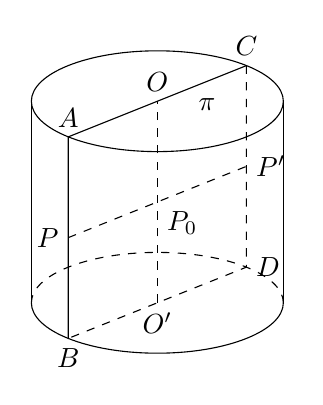
\begin{tikzpicture}[xscale=.8, yscale=.32]
\draw[dashed] (2,0) arc (0:180:2);
\draw (2,0) arc (0:-180:2);
\draw (0,8) circle (2);
\draw[dashed](1.414,1.414+8)--(1.414,1.414)node[right]{$D$}--(-1.414,-1.414);
\draw(1.414,1.414+8)node[above]{$C$}--(-1.414,-1.414+8)node[above]{$A$}--(-1.414,-1.414)node[below]{$B$};
\draw(-2,0)--(-2,8);\draw(2,0)--(2,8);
\node at (.5,.5+8)[below right]{$\pi$};
\draw[dashed](0,0)node [below]{$O'$}--(0,8)node [above]{$O$};
\draw[dashed](-1.414,-1.414+4)node[left]{$P$}--(1.414,1.414+4)node[right]{$P'$};
\node at (0,4)[below right]{$P_0$};
\end{tikzpicture}
    \caption{}
\end{figure}


\begin{proof}
\begin{enumerate}
    \item 

设点$P$是圆柱$AD$的柱面上
的任一点,过$P$作$PP_0\bot OO'$于$P_0$, 并且
$PP_0$的延长线交圆柱面于另一点$P'$。因为$PP'\cap OO'=P_0$, 所
以$PP'$、$OO'$确定一个平面$\pi$, $\pi$与圆柱面的交线为$AB$ ($P\in
AB$) 和$CD$ ($P'\in CD$), 与两底面的交线为$AC$ ($O\in AC$) 及
$BD$ ($O'\in BD$).

$\because\quad $圆柱的两个底面平行。

$\therefore\quad AC\parallel BD$ 且AC、BD分别为两底面圆的直径。

$\because\quad $圆柱的两底面是全等的圆面。

$\therefore\quad AC=BD\qquad ABDC$是平行四边形。

又$\because\quad AB$垂直两底面。

$\therefore\quad ABDC$为矩形,$\angle CAB=\angle ACD=90^{\circ}$

$\therefore\quad AO\displaystyle\mathop{=}^{\parallel}BO', OC\displaystyle\mathop{=}^{\parallel}O'D$

$\therefore\quad ABO'O$和$O'ODC$是两个全等的矩形

$\because\quad PP_0\bot OO'$于$P$.

$\therefore\quad PP_0=AO=OC=P_0P'$

$\therefore\quad PP'$被$OO'$垂直平分。

如果点$P$取在圆柱的底面上,那么它的像$P'$也在该圆面
上,同样可以证明$PP'$被$OO'$垂直平分。

$\therefore\quad OO'$是圆柱$AD$的对称轴。

\item 由1的证明可知,$OO'\parallel AB$, 而$AB$垂直于圆柱的两
个底面,所以$OO'$垂直于两底面。
\end{enumerate}
\end{proof}

\begin{blk}{定义}
    通过圆柱的轴的截面称为圆柱的轴截面。
\end{blk}

\begin{blk}{推论}
\begin{enumerate}
    \item 圆柱的轴截面是矩形。
    \item 过圆柱对称轴的平面是圆柱的对称平面。
    \item 平行于圆柱的轴的截面是矩形。
\end{enumerate}
\end{blk}

\begin{example}
    一圆柱用平行于圆柱的轴的平面去截它,截面周
界是30cm, 面积为54${\rm cm}^2$, 在底面上截得的一段弧为$120^{\circ}$, 求底面半径和圆柱的高。
\end{example}

\begin{figure}[htp]
    \centering
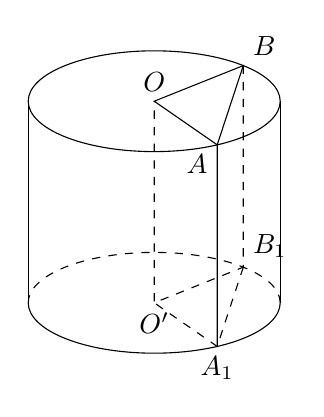
\begin{tikzpicture}[xscale=.8, yscale=.32]
\draw[dashed] (2,0) arc (0:180:2);
\draw (2,0) arc (0:-180:2);
\draw (0,8) circle (2);
\draw[dashed](1.414,1.414+8)node[above right]{$B$}--(1.414,1.414)node[above right]{$B_1$}--(0,0)node [below]{$O'$}--(0,8)node [above]{$O$};
\draw(-2,0)--(-2,8);\draw(2,0)--(2,8);
\draw[dashed](1.414,1.414)--(1,-1.732)node[below]{$A_1$}--(0,0);
\draw(1,-1.732)--(1,-1.732+8)--(0,8)--(1.414,1.414+8)--(1,-1.732+8)node[below left]{$A$};
\end{tikzpicture}
    \caption{}
\end{figure}

\begin{solution}
    如图2.10. 平行轴$OO'$的截面是矩形$AA_1B_1B$, 其边
$AB$是$\odot O$的弦,所对的圆心角是$120^{\circ}$, 故在$\triangle AOB$中,有
\[\frac{AB}{\sin 120^{\circ}}=\frac{R}{\sin 30^{\circ}}\]
其中$R$为$\odot O$的半径。

$\therefore\quad AB=\sqrt{3}R$

$\because\quad $矩形的另一边$AA_1$为圆柱的高,

$\therefore\quad AA_1=\frac{30}{2}-R\sqrt{3}$

又$\because\quad $矩形的面积为$54{\rm cm^2}$

$\therefore\quad R\sqrt{3}\left(15-R\sqrt{3}\right)=54 \quad \Rightarrow\quad R^2-5\sqrt{3}R+18=0$

解得:$R_1=3\sqrt{3},\quad R_2=2\sqrt{3}$,相应地圆柱高$h_1=6,\quad h_2=9$

答:圆柱底面半径为$3\sqrt{3}$cm, 高为
6cm, 或者半径为$2\sqrt{3}$cm, 高为9cm.
\end{solution}


\begin{ex}
\begin{enumerate}
    \item 柱面可视为准线沿母线方向连续平行移动时所占各位置
    的轨迹。用这句话说明棱柱、圆柱。
    \item 确定一个柱面需要几个条件?
    \item 从四棱柱、五棱柱和$n$棱柱的某一个顶点出发,各能引几
    条对角线?四棱柱、五棱柱和$n$棱柱各有几条对角线?
    \item \begin{enumerate}
    \item 平行六面体是斜四棱柱,斜四棱柱是不是平行六面
体?
\item 长方体是直四棱柱,直四棱柱是不是长方体?
\item 正方体是正四棱柱,正四棱柱是不是正方体?
    \end{enumerate} 

\item 有一个侧面是矩形的棱柱是不是直棱柱?有两个相对侧
面是矩形的$2n$棱柱呢?有两个相邻侧面是矩形的棱柱
呢?
\item 求证:和棱柱各侧棱相交的两个平行截面是两个全等的
多边形。
\item 求证:用平行于圆柱的底面的平面去截圆柱所得的截面
是和底面相等的圆面。
\item 一个圆柱体有多少个对称轴?有多少个对称平面?
\item 用第一种画法画正六棱柱的直观图,用第二种画法画圆
柱的直观图。
\end{enumerate}  
\end{ex}

\subsection{锥}

在前面我们初步地讨论了柱(包括棱柱和圆
柱)的定义及其某些性质。这一节将研究锥(包括棱锥和圆
锥)的定义及其性质,我们从锥面说起。

\subsubsection{锥面}

\begin{blk}
    {定义} 给定平面曲线$C$和$C$所在平面外一点$S$, 设直线$\ell$
经过$S$点运动并且总和$C$相交,则运动的直线$\ell$所产生的曲面
叫做锥面。$S$点叫做锥面的顶点,运动着的直线$\ell$的每一位置
叫作锥面的母线,而在运动中始终和母线相交的曲线$C$叫做
锥面的准线。
\end{blk}

通常,我们只讨论通过顶点$S$总和准线$C$相交的射线运
动时所产生的锥面。

下面我们来考虑几种简单情况:
\begin{enumerate}
    \item 准线是一条线段,这时锥面是一个平面区域,其边
    界是一个角。(图2.11)
    \item 准线是一个多边形,这时的锥面叫\textbf{多面角}。它是由
    从顶点出发通过多边形的各个顶点作射线,这些射线以及每
    两条相邻射线间平面部分所组成的图形。(图2.12)

    通过多边形顶点的母线叫作多面角的\textbf{棱}。锥面的顶点叫
    做多面角的\textbf{顶点}。相邻两棱的平面部分叫做多面角的\textbf{面},在
    每个面内由两条棱组成的角叫作多面角的\textbf{面角}。
    \item 准线是个圆,如果圆面垂直于连接顶点和圆心的直
    线,那么锥面叫作直圆锥面,简称圆锥面。(图2.13)通过
    顶点和准线圆中心的直线是圆锥面的轴。锥面的表示法可以
    用它的顶点字母$S$表示,记作锥面$S$. 也可表示成锥面$S-
    ABCDE$等其中$A,B,C,D,E$等分别是锥面上不同母线上的
    点。
\end{enumerate}

\begin{figure}[htp]\centering
    \begin{minipage}[t]{0.3\textwidth}
    \centering
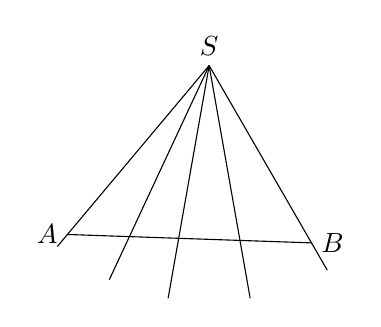
\begin{tikzpicture}[>=latex, scale=1]
    \foreach \x in {-60,-80,-100,-115,-130}
    {
        \draw(0,0)--(\x:3);
    }
    \node at (0,0)[above]{$S$};
    \draw(-130:2.8)node[left]{$A$}--(-60:2.6)node[right]{$B$};
    \end{tikzpicture}
    \caption{}
    \end{minipage}
    \begin{minipage}[t]{0.38\textwidth}
    \centering
    \begin{tikzpicture}[>=latex, scale=1]
\tkzDefPoints{0/0/A, 1.5/0/B, 2/.5/C, .8/1/D, -.5/.6/E, .8/2.5/S}
\draw(E)--(A)--(B)--(C);
\draw [dashed](C)--(D)--(E);
\tkzDrawLines[add=0 and .5](S,E S,A S,B S,C)
\tkzDrawLines[add=0 and 1, dashed](S,D)
\tkzLabelPoints[below](A,B)
\tkzLabelPoints[above](C,D,E,S)

    \end{tikzpicture}
    \caption{}
    \end{minipage}
    \begin{minipage}[t]{0.25\textwidth}
    \centering
    \begin{tikzpicture}[>=latex, yscale=.4]
        \draw[dashed] (1,0) arc (0:180:1);
        \draw (1,0) arc (0:-180:1);
\tkzDefPoints{1/0/A, -1/0/B, 0/6/S, 0/0/O}
\tkzDrawLines[add=0 and .5](S,A S,B)
\tkzDrawLines[add=0 and .35, dashed](S,O)
\draw(S)--+(-95:9);
\tkzLabelPoints[above](S,O)
    \end{tikzpicture}
    \caption{}
    \end{minipage}
    \end{figure}

\begin{blk}
    {定理} 不通过顶点$S$的两个平行平面与锥面相交,所
    得到的图形相似,其相似比等于顶点到两平行平面的距离之
    比。
\end{blk}

已知:锥面$S-ABC\cdots$, 平行平面$\alpha_1$与$\alpha_2$都不通过顶
点$S$与锥面相交,得到截面图形$F_1$(在$\alpha_1$上)与$F_2$(在$\alpha_2$上),
又$SO_1\bot\alpha_1$于$O_1$, $SO_2\bot\alpha_2$于$O_2$(图2.14)

求证:截面图形$F_1\backsim F_2$, 其相似比
$K=\frac{SO_1}{SO_2}$

\begin{figure}[htp]
    \centering
\includegraphics[scale=.6]{fig/2-14.png}
    \caption{}
\end{figure}

\begin{proof}
任引锥面$S-ABC\cdots$的一条母线$SX$, 由于$F_1$
和$F_2$都是锥面的截面,所以$SX$
必与$F_1$和$F_2$分别交于$X_1$和$X_2$两
点,这时,$X_2$可以看成$F_1$上$X_1$的
对应点,$X_1$也可看成是$F_2$上$X_2$
的对应点。

如果另外再取一条不同于
$SX$的母线$SY$, 同样可以得到
$F_1$和$F_2$上的另一对对应点$Y_1$和
$Y_2$, 显然$X_1\ne Y_1$, $X_2\ne Y_2$, 否
则$SX$与$SY$重合,这将与它们
是不同的母线相矛盾。因此,
$F_1$和$F_2$的点与点之间建立了一一对应关系。

又设$SX$和$SY$所确定的平面为$\pi$, 则$\pi\cap \alpha_1=X_1Y_1$,
$\pi\cap \alpha_2=X_2Y_2$, 因为$\alpha_1\parallel \alpha_2$, 所以$X_1Y_1\parallel X_2Y_2$. 因此:
\begin{equation}
    \frac{X_1Y_1}{X_2Y_2}=\frac{SX_1}{SX_2}
\end{equation}
连结$X_1O_1$, $X_2O_2$, 并令$SX$与$SO_2$所确定的平面为$\pi'$, 
则$\pi'\cap\alpha_1=X_1O_1$, $\pi'\cap\alpha_2=X_2O_2$

$\because\quad \alpha_1\parallel \alpha_2$

$\therefore\quad X_1O_1\parallel X_2O_2$
\begin{equation}
    \frac{SX_1}{SX_2}=\frac{SO_1}{SO_2}
\end{equation}
由(2.1), (2.2)有:
\[\frac{X_1Y_1}{X_2Y_2}=\frac{SO_1}{SO_2}=K\quad\text{(常数)}\]
由相似图形的定义可知:
\[F_1\backsim F_2,\quad \text{并且相似比}K=\frac{SO_1}{SO_2}\]
\end{proof}

\subsubsection{棱锥与圆锥}
\begin{blk}
   {定义} 如果一个锥面的准线是一条封闭曲线则称这个锥
面为封闭锥面。如圆锥面、多面角都是封闭锥面。

如果一个封闭锥面的所有线被一个平面所截,那么由
这个截面和锥面所围成的几何体叫做锥体。锥体平面部分叫
作锥体的底面,顶点和底面的距离叫做锥体的高。 
\end{blk}

下面我们讨论几个特殊的锥体。

\begin{blk}
    {定义}如果一个多面角的所有的棱被一个平面所截,那
么截面和多面角各面所围成的几何体叫作棱锥。原多面角的
顶点叫做棱锥的顶点,截面和多面角相交的部分显然是多边
形,它所围的平面部分叫做棱锥的底面,有公共顶点的各个
三角形的面叫做棱锥的侧面,两个相邻侧面的公共边叫做棱
锥的棱侧。

如果棱锥的底面是三角形、四边形……$n$边形,那么棱锥
就分别叫做\textbf{三棱锥,四棱锥,五棱锥……$n$棱锥}(见图2.15)、棱锥的表示法可以用表示顶点和底面顶点的
几个字母来表示,例如棱锥$S-ACD$. 
\end{blk}

如果棱锥的底面是正多边形,并且由棱锥顶点到它的底
面的垂线经过这个多边形的中心,那么这个棱锥就叫作\textbf{正棱
锥}。

\begin{figure}[htp]
    \centering
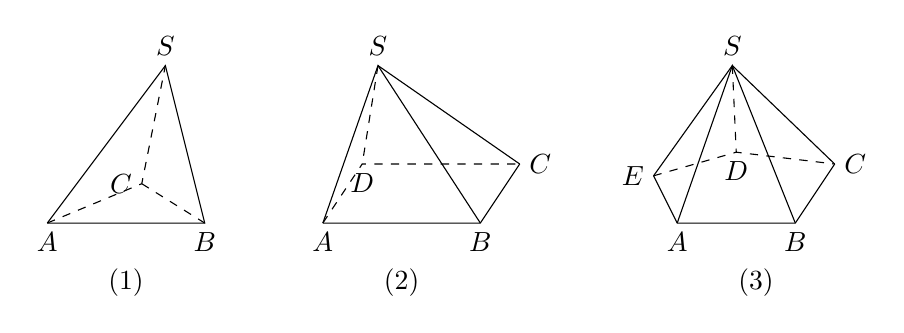
\begin{tikzpicture}
\begin{scope}
\draw(0,0)node[below]{$A$}--(2,0)node[below]{$B$}--(1.5,2)node[above]{$S$}--(0,0);
\draw[dashed](0,0)--(1.2,.5)node[left]{$C$}--(1.5,2);
\draw[dashed](1.2,0.5)--(2,0);
\node at (1,-.75){(1)};

\end{scope}
\begin{scope}[xshift=3.5cm]
    \draw(0,0)node[below]{$A$}--(2,0)node[below]{$B$}--(2.5,.75)node[right]{$C$};
\draw[dashed](0,0)--(.5,.75)node[below]{$D$}--(2.5,.75);
\draw(0,0)--(.7,2)node[above]{$S$}--(2,0);
\draw(.7,2)--(2.5,.75);
\draw[dashed](.7,2)--(.5,.75);
\node at (1,-.75){(2)};
\end{scope}
\begin{scope}[xshift=8cm]
    \draw(-.3,.6)node[left]{$E$}--(0,0)node[below]{$A$}--(1.5,0)node[below]{$B$}--(2,.75)node[right]{$C$};
    \draw(0,0)--(.7,2)node[above]{$S$}--(1.5,0);
    \draw(-.3,.6)--(.7,2)--(2,.75);

    \draw[dashed](-.3,.6)--(.75,.9)node[below]{$D$}--(2,.75);
\draw[dashed](.7,2)--(.75,.9);
    \node at (1,-.75){(3)};
\end{scope}
\end{tikzpicture}
    \caption{}
\end{figure}


图2.16是用第一种画法画出的正六棱锥的直观图。
\begin{figure}[htp]
    \centering
\includegraphics[scale=.55]{fig/2-16.png}
    \caption{}
\end{figure}

正棱锥显然有如下的性质:
\begin{enumerate}
\item 正棱锥所有的侧棱都相等。
\item 正棱锥过顶点的所有面角都相等。
\item 正棱锥各个侧面是全等的等腰三角形。

因为全等的等腰三角形底边上的高都相等,所以正棱锥侧面的等腰三角形底边上的高都叫作
正棱锥的\textbf{斜高}。例如图2.16(3)中$\triangle SBC$底边$BC$上的高$SG$就
是正棱锥$S-AD$的斜高。
\item 正棱锥所有的斜高都相等.
\item 正棱锥的棱、高、及棱在底上的射影以及斜高、高
和斜高在底面上的射影分别组成一个直角三角形。
\end{enumerate}

我们已经看到正棱锥的许多元素,如侧棱、底边(底面
正多边形的边)、高、斜高、侧棱和底面的夹角、侧面和底
面所成的角、斜高和高所成的角等等。在这些元素中只要给
出其中两个元素(至少有一线段),就可以通过解直角三角
形和底面正多边形来求出其它元素。

\begin{example}
已知棱锥底面是边长为12的三角形,它的各个侧
面和底面成$45^{\circ}$角,
\begin{enumerate}
    \item 求证这个棱锥是正三棱锥;
    \item 求这个三棱锥的高。
\end{enumerate}

已知:在棱锥$S-ABC$中,$AB=BC=CA=12$cm, 
面$SAB$、$SBC$、$SCA$都和底面$ABC$成$45^{\circ}$角.
\begin{enumerate}
    \item 求证:$S-ABC$是正三棱锥;
    \item 求三棱锥的高$SO$.
\end{enumerate}
\end{example}

\begin{solution}
    设$SO$为三棱锥的高,过$O$点在底面内作$OD$、$OE$、
$OF$分别垂直于$\triangle ABC$的各边$AB$、$BC$、$CA$, 连接$SD$、$SE$、
$SF$, 则$SD\bot BA$, $SE\bot BC$, $SF\bot AC$ (三垂线定理)(见图2.17), 即$\angle SDO$, $\angle SEO$, $\angle SFO$分别是棱锥各个侧
面和底面所成二面角的平面角。

$\therefore\quad \angle SDO=\angle SEO=\angle SFO=45^{\circ}$

从而$\triangle SOD\cong \triangle SOE\cong \triangle SOF$,
于是$OD=OE=OF$。

即:$O$点是$\triangle ABC$的内心,又因为正三角形的内心、外
心、重心、垂心重合,所以三棱锥$S-ABC$是正三棱锥。

又$OD=\frac{1}{3}CD=\frac{1}{3}\sqrt{CB^2-BD^2}=\frac{1}{3}\sqcup12^2-6^2=\frac{1}{3}\x 6\sqrt{3}=2\sqrt{3}$

$\because\quad \triangle SOD$是等腰直角三角形

$\therefore\quad SO=OD=2\sqrt{3}$ (cm)

答:棱锥的高为$2\sqrt{3}$cm.
\end{solution}

\begin{figure}[htp]\centering
    \begin{minipage}[t]{0.48\textwidth}
    \centering
\begin{tikzpicture}
\tkzDefPoints{0/0/A, 3/0/B, 4/1.5/C, 2/3/S, 2.3/.5/O}
\tkzDefMidPoint(A,B) \tkzGetPoint{D}
\tkzDefMidPoint(A,C) \tkzGetPoint{F}
\tkzDefMidPoint(C,B) \tkzGetPoint{E}
\tkzDrawSegments(A,B B,C S,A S,B S,C S,D S,E)
\tkzDrawSegments[dashed](A,C S,F F,B C,D A,E S,O)
\tkzLabelPoints[below](A,D,B,O)
\tkzLabelPoints[right](E,C)
\tkzLabelPoints[above](F,S)

\end{tikzpicture}
    \caption{}
    \end{minipage}
    \begin{minipage}[t]{0.48\textwidth}
    \centering
\begin{tikzpicture}[yscale=.4]
\tkzDefPoints{1.5/0/C, -1.5/0/A, 0/8/S, 0/0/O}
\tkzDefPoint(-45:1.5){D}
\tkzDefPoint(-45-90:1.5){B}
\draw[dashed](1.5,0) arc (0:180:1.5);
\draw(1.5,0) arc (0:-180:1.5);

\tkzDrawSegments(S,D S,B S,A S,C)
\tkzDrawSegments[dashed](D,O S,O B,O)
\tkzLabelPoints[below](D,B,O)
\tkzLabelPoints[above](S)
\tkzLabelPoints[left](A)
\tkzLabelPoints[right](C)
\node at (0,4) [right]{$h$};
\node at (-.5,3.5) [left]{$\ell$};
\node at (-135:0.5)[left]{$r$};

\end{tikzpicture}
    \caption{}
    \end{minipage}
    \end{figure}

\begin{blk}
    {定义} 如果用不经过圆锥面顶点而垂直于圆锥面的轴的
一个平面去截圆锥面,那么截面和圆锥面所围成的几何体叫
做直圆锥,简称圆锥(图2.18)。原来圆锥面的顶点和轴分别
叫做圆锥的顶点和轴,圆锥面母线夹在顶点和截面之间的部
分叫做圆锥的母线。圆锥面夹在顶点和截面之间的部分叫作
圆锥的侧面。圆锥可以用它的顶点以及它的底面上三个点的
字母来表示,如图2.18的圆锥可以记作圆锥$S-ABC$, 也可
以简记作圆锥$S$.
\end{blk}

圆锥也可以看成是以直角三角形
的一条直角边所在直线为轴,直角
三角形旋转一周而成的几何体。例
如以直角三角形$SOB$的一条直角边
所在的直线为轴,使$\triangle SOB$旋转一
周,$OB$、$SB$旋转所成的面就围成了一
个圆锥(图2.18),直角边$SO$叫做圆
锥的高,直角边$OB$旋转而成的圆面叫做圆锥的底面,斜边
旋转而成的面叫做圆锥的侧面,在侧面各个位置的斜边叫做
圆锥的母线。显然圆锥的任一条母线$\ell$和高$h$, 以及这条母
线$\ell$在底面上的射影即底面半径$r$组成一个直角三角形,根据
勾股定理有:
\[\ell^2=h^2+r^2\]

圆锥有下面的一些性质:
\begin{enumerate}
\item 圆锥的母线都经过顶点并且都相等。
\item 各母线和轴的夹角相等。
\item 垂直于圆锥的轴而且不经过圆锥顶点的平面去截圆
锥面,所得的截面是圆面。因此截面圆与底面圆相似。
\item 过轴的平面是圆锥的对称平面。
\item 过轴的所有截面是全等的等腰三角形。
\end{enumerate}


\begin{example}
求证:与圆锥底面圆相切的直线,和过切点所作的
母线互相垂直。

已知:圆锥$V-ABC$, 底面圆的切线$AT$, 母线$VA$
(图2.19)

\begin{figure}[htp]
    \centering
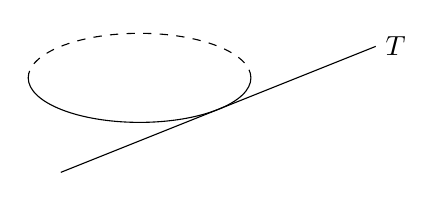
\begin{tikzpicture}[yscale=.4]
\draw[dashed](0.414,1) arc (0:180:1.414);
\draw(0.414,1) arc (0:-180:1.414);
\tkzDefPoints{0.414/1/B, -2.414/1/C, -1/9/V, 0/0/A,-1/1/O}
\draw(2,2)node[right]{$T$}--(-2,-2);
\tkzDrawSegments(V,C V,A V,B)
\tkzDrawSegments[dashed](V,O O,A)
\tkzLabelPoints[above](V)
\tkzLabelPoints[left](C,O)
\tkzLabelPoints[below right](A)
\tkzLabelPoints[right](B)
\end{tikzpicture}
    \caption{}
\end{figure}

求证:$AT\bot VA$
\end{example}

\begin{proof}
设$O$为圆锥底面的圆心,连接
$VO$、$OA$, 则$VO\bot$平面$ABC$.

$\therefore\quad VA$在平面$ABC$上的射影是$OA$.

$\because\quad AT$是$\odot O$的切线,

$\therefore\quad OA\bot AT$

由三垂线定理,有$AT\bot VA$.
\end{proof}

\begin{ex}
\begin{enumerate}
    \item \begin{enumerate}
        \item 底面是正多边形的棱锥是正棱锥吗?
    \item 侧棱都相等的棱锥是正棱锥吗?
    \item 侧面和底面夹角都相等的棱锥是正棱锥吗?
    \end{enumerate}
  
    \item 
    \begin{enumerate}
      \item 棱锥的侧棱和底面所成的角都相等,则顶点在底面
    上的射影是什么?
    \item 棱锥的侧面和底面所成的二面角都相等,则顶点在
    底面上的射影是什么?  
    \end{enumerate}
    
    \item 证明:六条棱长相等三棱锥是正三棱锥。
    \item 试用两种画法分别画出底面边长为6cm, 高为15cm的
    正六棱锥的直观图,比例尺为
    \item 用第二种画法画出底面半径是2cm, 母线为3cm的圆锥的
    直观图。
    \item 用第一种画法画出底面边长为2cm, 高为4cm的正五棱
    的直观图。
    \item 在正六棱锥$V-ABCDEF$中,底面多边形的边长为$a$,
    侧棱长为$2a$, 求这棱锥的高$VO$及斜高$VM$的长。
    \item 已知圆锥底面圆的半径为3cm, 高为4cm, 设$VA$是圆锥
    的一条母线,$O$点是底面中心,如果$OM\bot VA$于$M$, 求
    $OM$的长。
\end{enumerate}
\end{ex}

\subsection{台体}
\begin{blk}{定义}
    平行于棱锥底面的平面与棱锥侧面相截,棱锥在
底面和截面之间的部分叫做棱台。原棱锥的底面和截面叫做
棱台的下底面和上底面,其他各面叫侧面,两相邻侧面的公
共边叫做棱台的侧棱,两个底面之间的距离叫做棱台的高。
(图2.20)
\end{blk}

\begin{figure}[htp]
    \centering
\begin{tikzpicture}[scale=1.3]
\begin{scope}
    \tkzDefPoints{0/0/A, 2/0/B, 2.75/.75/C, .75/.75/D, 1.375/3/S, 1.375/.375/O}
    \tkzDefMidPoint(S,A) \tkzGetPoint{A'}
    \tkzDefMidPoint(S,B) \tkzGetPoint{B'}
    \tkzDefMidPoint(S,C) \tkzGetPoint{C'}
    \tkzDefMidPoint(S,D) \tkzGetPoint{D'}
    \tkzDefMidPoint(S,O) \tkzGetPoint{O'}
    \tkzDrawPolygon(A',B',C',D')
    \tkzDrawSegments(A,B B,C A,A' B,B' C,C')
    \tkzDrawSegments[dashed](A',S B',S C',S O,S A,D C,D S,D)
    \tkzLabelPoints[below](A,B)
    \tkzLabelPoints[left](A',D',D)
    \tkzLabelPoints[right](C,C',B',O,O')

\node at (1.5,-.5){(1)};
\end{scope}
\begin{scope}[xshift=5cm]
    \tkzDefPoints{0/0/A, 2/0/B, 2.75/.75/C, .75/.75/D, 1.375/3/S, 1.375/.375/O}
\tkzDefMidPoint(S,A) \tkzGetPoint{A'}
\tkzDefMidPoint(S,B) \tkzGetPoint{B'}
\tkzDefMidPoint(S,C) \tkzGetPoint{C'}
\tkzDefMidPoint(S,D) \tkzGetPoint{D'}
\tkzDrawPolygon(A',B',C',D')
\tkzDrawSegments(A,B B,C A,A' B,B' C,C')
\tkzDrawSegments[dashed](A,D C,D D',D)
\node at (1.5,-.5){(2)};
\end{scope}
\end{tikzpicture}
    \caption{}
\end{figure}


棱台可以用表示上、下底顶点的字母来表示,例如棱台
$AC'$. 也可记作棱台$ABCD-A'B'C'D'$(图2.20(1)).

由三棱锥、四棱锥、五棱锥……截得的棱台分别叫做\textbf{三
棱台、四棱台、五棱台}……

\begin{blk}
{定义} 由正棱锥截得的棱台叫做正棱台。    
\end{blk}



\begin{figure}[htp]
    \centering
\begin{tikzpicture}[scale=1.3]
\begin{scope}
    \tkzDefPoints{-.5/0/A, .5/0/B, -1.1/.4/E, 1.1/.4/C, 0/.8/D, 0/2.5/S}
    \tkzDefMidPoint(S,A) \tkzGetPoint{A'}
    \tkzDefMidPoint(S,B) \tkzGetPoint{B'}
    \tkzDefMidPoint(S,C) \tkzGetPoint{C'}
    \tkzDefMidPoint(S,D) \tkzGetPoint{D'}
    \tkzDefMidPoint(S,E) \tkzGetPoint{E'}
    \tkzDrawPolygon(A',B',C',D',E')
    \tkzDrawSegments(A,B B,C E,A A,A' B,B' C,C' E,E')
    \tkzDrawSegments[dashed](A',S S,E'  B',S C',S  C,D E,D)
    
    \node at (0,-.5){(1)};

\end{scope}
\begin{scope}[xshift=3cm]
    \tkzDefPoints{0/0/A, 2/0/B, 2.75/.75/C, .75/.75/D, 1.375/3/S, 1.375/.375/O, 2.375/.375/E}
\tkzDefMidPoint(S,A) \tkzGetPoint{A'}
\tkzDefMidPoint(S,B) \tkzGetPoint{B'}
\tkzDefMidPoint(S,C) \tkzGetPoint{C'}
\tkzDefMidPoint(S,D) \tkzGetPoint{D'}
\tkzDefMidPoint(S,E) \tkzGetPoint{E'}
\tkzDefMidPoint(S,O) \tkzGetPoint{O'}
\tkzDrawPolygon(A',B',C',D')
\tkzDrawSegments(A,B B,C A,A' B,B' C,C' E,E')
\tkzDrawSegments[dashed](A,D C,D D',D O,O' O,E O',E' O,B O',B')
\node at (1.5,-.5){(2)};
\end{scope}
\end{tikzpicture}
    \caption{}
\end{figure}

正棱台有下面一些性质:
\begin{enumerate}
\item 正棱台的两个底面及平行于底面的截面是相似的正
多边形。(图2.21)
\item 两底面中心连线垂直于底面(图2.21(2))。
\item 正棱台的各侧面是全等的等腰梯形,各等腰梯形的
高相等,它叫做正棱台的斜高。(图2.21(2))
\item 正棱台的各侧棱相等,并且延长后相交于一点。
(图2.21(1))
\item 正棱台两底面中心连线、相应的两底面的边心距和
斜高组成直角梯形;两底中心连线、侧棱和两底面相应的半
径组成一个直角梯形;同一个侧面上的上底和下底中点的连
线将这个侧面分成两个全等的直角梯形。(见图2.21(2))
\end{enumerate}

解正棱台的问题一般总可化为解5中提到的直角梯形
及底面的正多边形的问题。

\begin{example}
    设正三棱台的两个底面边长分别是2cm和5cm, 侧
棱长为5cm, 求这个棱台的高和斜高(图2.22)。
\end{example}

\begin{figure}[htp]
    \centering
\begin{tikzpicture}[scale=1.2]
\tkzDefPoints{0/0/A, 4/0/C, 3/-1.5/B, 2.5/3/S, 2.5/-.45/O, 1.5/-.75/D}
\tkzDefMidPoint(S,A) \tkzGetPoint{A_1}
\tkzDefMidPoint(S,B) \tkzGetPoint{B_1}
\tkzDefMidPoint(S,C) \tkzGetPoint{C_1}
\tkzDefMidPoint(S,O) \tkzGetPoint{O_1}
\tkzDefMidPoint(S,D) \tkzGetPoint{D_1}

\tkzDrawPolygon(A_1,B_1,C_1)
\tkzDrawSegments(A,B B,C A,A_1 B,B_1 C,C_1 A_1,O_1 O_1,D_1 D_1,D)
\tkzDrawSegments[dashed](O,D A,C A,O O,O_1)

\tkzLabelPoints[left](A,A_1,D_1)
\tkzLabelPoints[right](C,C_1,O,O_1,B_1)
\tkzLabelPoints[below](B,D)
\tkzDefPointsBy[translation = from O_1 to D_1](O){F}
\tkzDefPointsBy[translation = from O_1 to A_1](O){E}
\tkzDrawSegments[dashed](D_1,F A_1,E)
\tkzLabelPoints[below](E,F)



\end{tikzpicture}
    \caption{}
\end{figure}


\begin{solution}
设两底面的中心分别为$O_1$和$O$, 连接$O_1O$, $O_1A_1$,
 $OA$. 取$A_1B_1$的中点$D_1$, $AB$的中
点$D$, 连接$O_1D_1$, $OD$, $D_1D$. 则
$O_1O$是棱台的高,$DD_1$是棱台的
斜高;并知$O_1A_1AO$和$OO_1D_1D$是两个直角梯形。分别引$A_1E\bot
AO$于$E$, $D_1F\bot DO$于$F$. 

由于上、下两底的边长分
别为2cm和5cm.

因此:
\[O_1A_1=\frac{\sqrt{3}}{3}\x 2=\frac{2}{3}\sqrt{3}, \qquad  OA=\frac{\sqrt{3}}{3}\x 5=\frac{5}{3}\sqrt{3}\]
因此:$AE=OA-O_1A_1=\frac{5}{3}\sqrt{3}-\frac{2}{3}\sqrt{3}=\sqrt{3}$


在直角$\triangle AA_1E$中,
\[A_1E=A_1A_2-AE_2=\sqrt{5^2-(\sqrt{3})^2}=\sqrt{22}\approx 4.69\]

$\therefore\quad OO_1=A_1E=\sqrt{22}\approx 4.69$(cm)

又$\because\quad O_1D_1=\frac{\sqrt{3}}{6}\x 2=\frac{\sqrt{3}}{3},\qquad OD=\frac{\sqrt{3}}{6}\x 5=\frac{5}{6}{\sqrt{3}}$

$\therefore\quad DF=OD-O_1D_1=\frac{5}{6}{\sqrt{3}}-\frac{\sqrt{3}}{3}=\frac{\sqrt{3}}{2}$

在直角$\triangle DD_1F$中
\[\begin{split}
    D_1D&=\sqrt{DF^2+D_1F^2}=\sqrt{DF^2+O_1O^2}\\
&=\sqrt{\left(\frac{\sqrt{3}}{2}\right)^2+(\sqrt{22})^2}=\frac{1}{2}\sqrt{91}\approx 4.77({\rm cm})
\end{split}\]

答:这棱台的高约等于4.69cm, 斜高约等于4.77cm.
\end{solution}

\begin{blk}
    {定义} 平行于圆锥底面的平面与圆锥相截,圆锥的底面
和截面之间的部分叫做圆台。原来圆锥的底面和截面分别叫
做圆台的下底面和上底面,原来圆锥的轴叫做圆台的轴,原
来圆锥的母线夹在两底面之间的部分叫做圆台的母线,原来
圆锥的侧面夹在两底面之间的部分叫做圆台的侧面,两底面
之间的距离叫做圆台的高。(图2.23)
\end{blk}

圆台也可以看作是一个直角梯形绕着垂直于底边的一条
腰所在的直线为轴,旋转$360^{\circ}$时,这个直角梯形的两底边及
另一腰所形成的面围成的几何体。直角梯形的上、下两底边旋
转而成的圆面分别叫做圆台的上底面和下底面。直角梯形垂
直于底边的腰的长叫做圆台的高,而另一腰则称为圆台的母
线。(图2.24)

\begin{figure}[htp]\centering
    \begin{minipage}[t]{0.48\textwidth}
    \centering
\begin{tikzpicture}[>=latex, yscale=.4]
\tkzDefPoints{-1.5/0/A_1, 1.5/0/C_1, -1/4/A, 1/4/C, 0/0/O_1, 0/4/O, 0/12/S}
\tkzDefPoint(-120:1.5){B_1}
\draw(O) circle (1);
\draw(C_1) arc (0:-180:1.5);
\draw(C_1)[dashed] arc (0:180:1.5);
\tkzDrawSegments(A,A_1 C,C_1)
\tkzDrawSegments[dashed](A,S C,S S,O_1 S,B_1)
\tkzLabelPoints[left](A,A_1)
\tkzLabelPoints[right](C,C_1,O,O_1)
\tkzLabelPoints[below](B_1)
\tkzInterLC(S,B_1)(A,C) \tkzGetPoints{B'}{B}
\tkzDrawLines[add=0 and .3](B_1,B) \tkzLabelPoints[right](B)
\tkzLabelPoints[above](S)
    \end{tikzpicture}
    \caption{}
    \end{minipage}
    \begin{minipage}[t]{0.48\textwidth}
    \centering
    \begin{tikzpicture}[>=latex, yscale=.4]
        \tkzDefPoints{-1.5/0/A_1, 1.5/0/C_1, -1/4/A, 1/4/C, 0/0/O_1, 0/4/O, 0/12/S}
        \tkzDefPoint(-120:1.5){B_1}
\draw(O) circle (1);
\draw(C_1) arc (0:-180:1.5);
\draw(C_1)[dashed] arc (0:180:1.5);
\tkzDrawSegments(A,A_1 C,C_1)
\tkzDrawSegments[dashed](O,O_1 O_1,C_1)
\tkzDrawSegments(C_1,C O,C) 
\tkzLabelPoints[left](O, O_1)
\node at (C)[right]{$A$};
\node at (C_1)[right]{$B$};
\node at (.5,4)[above]{$R_1$};
\node at (.75,0)[above]{$R_2$};
    \end{tikzpicture}
    \caption{}
    \end{minipage}
    \end{figure}


圆台的表示法是用它两底上而不在同一条母线上的两个
点的字母来表示。如图2.23的圆台可以记作圆台$AB_1$.

圆台有下面一些性质:
\begin{enumerate}
\item 圆台的两个底面是圆,它们所在的平面平行。
\item 圆台的轴经过两个底面的圆心,并且和底面垂直,
连结两底圆心线段的长等于高。
\item 圆台的母线都相等。
\item 圆台的各母线的延长线交于一点。
\item 经过圆台的轴的截面叫圆台的轴截面,它是一个等
腰梯形。
\item 经过圆台的轴的平面是圆台的对称平面。
\end{enumerate}

如果设圆台的上、下两底面的半径分别为$R_1$和$R_2$, 母线
长为$\ell$, 高为$h$, 那么$\ell^2=(R_2-R_1)^2+h^2$ (图2.24)

\begin{example}
    已知一个圆台两底面面积分别是$1{\rm dm^2}$和$49{\rm dm^2}$, 有
    一个截面和底面平行,它的面积是$25{\rm dm^2}$, 求这个截面和两
    个底面距离的比。
\end{example}

\begin{figure}[htp]
    \centering
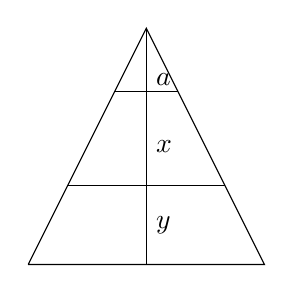
\begin{tikzpicture}[scale=.5]
\draw(-3,0)--(3,0)--(0,6)--(-3,0);
\draw(-2,2)--(2,2);
\draw(-1+.2,4+.4)--(1-.2,4+.4);
\draw(0,0)--(0,6);
\node at (0,1) [right]{$y$};
\node at (0,3) [right]{$x$};
\node at (0,4.7) [right]{$a$};
\end{tikzpicture}
    \caption{}
\end{figure}

\begin{solution}
    设从截得圆台的原来圆锥的顶点到圆台上底的距离
是$a$ $(a>0)$, 从截面到圆台上底面和下底
面的距离分别是$x$和$y$, 那么参看轴截面
图2.25,由圆台的性质及相似形面积的比等于相似比的平方,就得到
\[\frac{(a+x)^2}{a^2}=\frac{25}{1},\qquad \frac{(a+x+y)^2}{a^2}=\frac{49}{1}\]
由此得正数解$x=4a$, $y=2a$。因此,$x:y=4a:2a=2:1$

答:截面和上、下两底面距离的比为2:1.
\end{solution}



\begin{ex}
\begin{enumerate}
    \item 如果两个相似三角形(不在同一平面内)的对应边互相
    平行,连结它们的对应顶点而形成各面所围成的几何体
    是不是棱台。
    \item 已知正棱台上、下两底面的边长分别是$a$和$b$ $(a<b)$, 侧
    棱和底面成$45^{\circ}$角,求它的侧棱和斜高的长。
    \item 圆台的两底面半径分别是$r_1$和$r_2$ ($r_1>r_2$), 母线与底面夹
    角是$60^{\circ}$, 求它的高。
    \item 圆台的母线长为$2a$, 母线与轴的夹角为$30^{\circ}$,一个底面半径是另一个底面半径的2倍,求两底面的半径。
    \item 下图是正四棱台的二视图,
    (图中所标尺寸单位是cm)
    试用两种画法画出它的直观
    图,比例尺为
    1/3.
\end{enumerate}
\end{ex}

\begin{figure}[htp]
    \centering
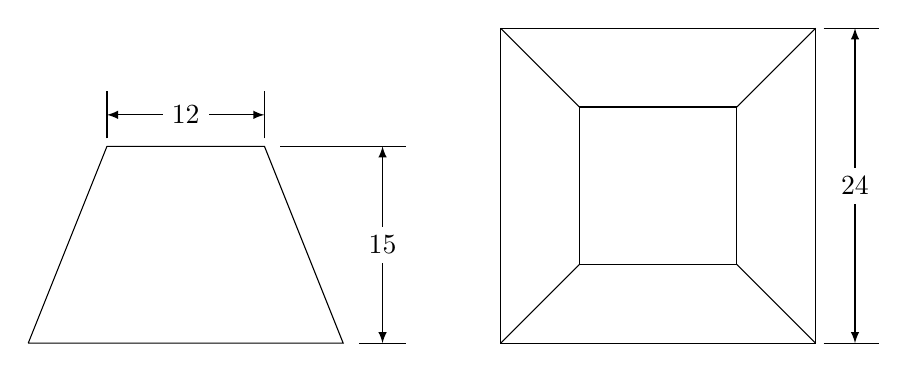
\begin{tikzpicture}[>=latex]
\begin{scope}
\draw(0,0)--(4,0)--(3,2.5)--(1,2.5)--(0,0);
\draw[<->](3,2.9)--node[fill=white]{12}(1,2.9);
\draw[<->](4.5,0)--node[fill=white]{15}(4.5,2.5);
\draw(4.2,0)--(4.8,0);
\draw(3.2,2.5)--(4.8,2.5);
\draw(1,2.6)--(1,3.2);
\draw(3,2.6)--(3,3.2);
\end{scope}
\begin{scope}[xshift=6cm]
\draw(0,0) rectangle(4,4);
\draw(1,1) rectangle(3,3);
\draw[<->](4.5,0)--node[fill=white]{24}(4.5,4);
\draw(1,1)--(0,0);
\draw(3,3)--(4,4);\draw(3,1)--(4,0);
\draw(1,3)--(0,4);
\draw(4.1,0)--(4.8,0);
\draw(4.1,4)--(4.8,4);
\end{scope}
\end{tikzpicture}
    \caption*{第5题}
\end{figure}

\subsection{球}

\begin{blk}
    {定义} 在空间与定点距离相
的点的集合称做球面。球面所
包围的立体叫做球。定点叫做球
心,定点和球面上任一点所连线
段叫做球的半径。连结球面上任意两点的线段叫做球的弦,
通过球心的弦叫做球的直径。
\end{blk}

球面也可以看作半圆绕着它的直径旋转一周所成的图
形。球可以看作是一半圆面绕着它的直径旋转一周而形成的
立体。原半圆面的半径是球的半径,原半圆面的圆心是球
心。

一个球可以用表示它球心的字母来表示,例如“球$O$”。
画半径是$R$的直观图时,一般用第二种画法,先分别在$XOY$、
$XOZ$、$YOZ$三个平面的画出表示半径是$R$的圆的三个椭圆,再
在外面画一个圆和这三个椭圆相切(图2.26),通常用简便
的画法如图2.27.

\begin{figure}[htp]\centering
    \begin{minipage}[t]{0.48\textwidth}
    \centering
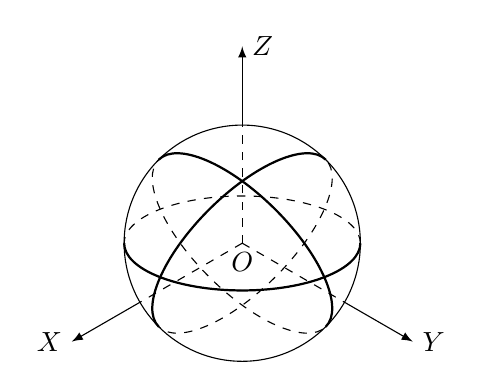
\begin{tikzpicture}[>=latex, scale=1]
\draw(0,0) circle(1.5);
\foreach \x in {90,-30,-150}
{
    \draw[dashed](0,0)--(\x:1.5);
    \draw[->](\x:1.5)--(\x:2.5);
}

\node at (90:2.5)[right]{$Z$};
\node at (-30:2.5)[right]{$Y$};
\node at (-150:2.5)[left]{$X$};
\node at (0,0)[below]{$O$};
\draw[dashed](0,0) ellipse [x radius=1.5, y radius= .6, rotate=45];
\draw[dashed](0,0) ellipse [x radius=1.5, y radius= .6, rotate=-45];
\draw[dashed](0,0) ellipse [x radius=1.5, y radius= .6];
\draw[thick](-1.5,0) arc [x radius=1.5, y radius= .6, start angle=180, delta angle=180];
\draw[thick, rotate=45](-1.5,0) arc [x radius=1.5, y radius= .6, start angle=180, delta angle=-180];
\draw[thick, rotate=-45](-1.5,0) arc [x radius=1.5, y radius= .6, start angle=180, delta angle=-180];
    \end{tikzpicture}
    \caption{}
    \end{minipage}
    \begin{minipage}[t]{0.48\textwidth}
    \centering
    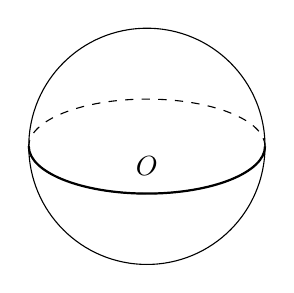
\begin{tikzpicture}[>=latex, scale=1]
        \draw(0,0) circle(1.5);  
        \draw[dashed](0,0) ellipse [x radius=1.5, y radius= .6];
        \draw[thick](-1.5,0) arc [x radius=1.5, y radius= .6, start angle=180, delta angle=180];
        \node at (0,0)[below]{$O$};
        \tkzDrawPoint(0,0)
    \end{tikzpicture}
    \caption{}
    \end{minipage}
    \end{figure}



球有下列一些性质:
\begin{enumerate}
    \item 同球的半径(或直径)相等。
    \item 球被平面所截得截面是一圆面。
\end{enumerate}

\begin{figure}[htp]
    \centering
\includegraphics[scale=.7]{fig/2-28.png}
    \caption{}
\end{figure}

\begin{proof}
    设平面$M$通过球心$O$, 并设$A$、$B$为平面$M$和球面交线
    上任意两点。(图2.28(1))在平面$M$内连接$OA$, $OB$, 因
    $OA$、$OB$都是球$O$的半径,所以$OA=OB$. 这就是说,交线上
    任意两点,因为交线上一切点与$O$点等距离,所以交线是平
    面$M$内以$O$点为圆心的一个圆,它的半径就等于球的半径,
    因此球$O$与平面$M$的截面是以球心为圆心的圆面。

设平面$M$不通过球心(图2.28(2)),自球心$O$作$OO_1$
    垂直平面$M$于$O_1$, 设$A$、$B$为平面$M$与球$O$的交线上任意两点,
    连结$OA$, $OB$, 因为$OA=OB$, 所以它们在平面$M$内的射影相
    等,即$AO_1=BO_1$, 因此平面$M$与球$O$的交线是一个圆,它的圆
    心就是球心$O$到平面的垂线的垂足$O_1$. 如果用$R,r$分别表示球
    的半径和截面圆的半径,$d$表示由球心$O$到平面$M$的距离,
那么,
\[r=\sqrt{R^2-d^2}\]
因此,平面$M$和球$O$的截面是以$O_1$为圆心,以$\sqrt{R^2-d^2}$
为半径的圆面。
\end{proof}

\begin{blk}{推论}
\begin{enumerate}
\item 连结球心与截面圆的圆心的直线和截面垂直。
\item 与球心距离相等的截面的圆大小相等。
\item 与球心距离不等的截面,所截得的圆的大小不等,距
离球心较近的截面所截的圆较大。
\item 当$d=0$时,这时截面过球心,所以$r=R$, 也就是说,
这时截面的圆的半径最大,称这个圆为球的大圆,不过球心
截面的圆称为球的小圆。
\item 当$d=R$时,$r=0$, 这时截面的圆退化为一个点,我们
称和球面只有一个公共点的乎面叫做球的切面,球的切面和
球的公共点叫做切点。和球只有一个公共点的直线叫做球的
切线。显然在球的切面上过切点的直线是球的切线。
\end{enumerate}
    
\end{blk}

\begin{blk}{定义} 
    连结球面上$A$、$B$两点间大圆的劣孤叫做球面上
$A$、$B$两点间的球面距离。
\end{blk}

\begin{blk}
    {定理} 如果球的半径通过球面
    的切面的切点,这个半径必垂直于
    球的切面。
\end{blk}


































\subsection*{习题2.1}

\begin{enumerate}
    \item \begin{enumerate}
        \item 图示四棱柱、平行六面体、直平行六面体、长方
    体、正方体各集合之间的关系。
    \item 图示多面体、凸多面体、棱柱、棱锥、棱台、平
    行六面体各集合之间的关系。
    \end{enumerate}
   
    \item 已知长方体的对角线与其共顶点的三条棱分别成角$\alpha,\beta,\gamma$,求证:
    \[\cos^2\alpha+\cos^2\beta+\cos^2\gamma=1\]
    \item 已知长方体的一条对角线与各个面所成的角分别是$\alpha,\beta,\gamma$,求证:\[\cos^2\alpha+\cos^2\beta+\cos^2\gamma=2\]
    \item 四棱柱的对角线如果交于一点,求证:此柱是平行六面
    体。
    \item 底面是菱形的直棱柱对角线长分别是9cm和15cm, 侧棱
    是5cm, 求它的底面边长。
    \item 在直平行六面体$ABCD-A_1B_1C_1D_1$中,若$AD=1$m,
    $AB=2$m, $AA_1=3$m, $\angle DAB=60^{\circ}$,求对角线$BD_1$和$AC_1$
    的长。
    \item 圆柱有一个内接直三棱柱,直三棱柱的一个侧面经过连
    结圆柱两底中心的轴,求证:直三棱柱的其他两侧面互
    相垂直。
    \item 已知正六棱锥的底面边长是4cm, 侧棱长是8cm, 求它
    的侧面和底面所成的角。
    \item 四面体(三棱锥)的各顶点与其对面的重心的连线共有
    四条,试证这四条直线交于一点。

    \item 试证:平行六面体所有对角线交于一点,而且互相平
分。
\item 求证:正三棱锥的侧棱与底面的对边垂直。
\item 如果棱锥的侧棱相等且侧面和底面成相等的角,求证:
这个棱锥是正棱锥。
\item 如果一个正三棱锥在顶点处的三个面角都是直角,求它
的侧棱与底面所成的角。
\item 一个正三棱锥的底面边长为$a$, 侧棱和底面成$\alpha$角,求这
棱锥的高和斜高。
\item 正三棱柱的棱长及底面边长都是$a$, 过底面一边及其相
对侧棱的中点作截面,求此截面的面积。
\item 过长方体$ABCD-A_1B_1C_1D_1$的底面一条对角线$AC$作一
个平面平行于长方体的一条对角线$BD_1$, 如果长方体的
底面是一个边长为$a$的正方形,对角线$BD_1$和底面所成
的角为$\alpha$, 求这个截面的面积。
\item 圆锥的高为20cm, 过圆锥的顶点与底面成$45^{\circ}$角的平
面,把圆锥底面圆周截成1:3两部分,求截面的面积。
\item 在一个正棱锥中,求证:
\begin{enumerate}
    \item 各条侧棱与底面所成的角都相等。
    \item 各侧面和底面所成的二面角相等。
\end{enumerate}

\item 已知正四棱锥的侧棱为15, 侧棱与底面所成的角为$45^{\circ}$,
画出正四棱锥的二视图与直观图。
\item 已知圆锥底面半径为4cm, 母线与底面所成的角为$60^{\circ}$,
求圆锥内接正四棱锥的斜高。
\item 正六棱锥$S-ABCDEF$的侧棱为$4a$, 底面正六边形边长
为$a$, 求过$SA$和$SC$的对角面的面积。
\item 正三棱台的上、下两底的边长分别为2cm和6cm, 侧棱
和底面成$60^{\circ}$角,求棱台的高和斜高。
\item 正四棱台的上下底的边长是6cm和24cm, 斜高为15cm, 
求这棱台的高。
\item 圆台的高为$h$, 母线和底面成$30^{\circ}$角,求母线的长。
\item 正四棱台上、下两底边长分别为$a$和$b$ ($a<b$), 侧棱和
底面成$45^{\circ}$角,求它的侧棱和斜高。
\item 圆台的高是两个底面的面积分别是$3\pi h^2$和$12\pi h^2$, 求圆
台的母线和底面所成的角。
\item 台体上、下两底的面积各是$Q_1$和$Q_2$, 求证这台体的高
和截得这台体的原锥体高的比是
\[\frac{Q_2-\sqrt{Q_1\cdot Q_2}}{Q_2}\]
\item 台体的两底面积分别是$9{\rm cm^2}$和$25{\rm cm^2}$, 求它的中截面的
面积。
\item 求证:球的任意两个大圆互相平分。
\item 在半径是13cm的球面上,有$A,B,C$三点,$AB=6$cm, 
$BC=8$cm, $CA=10$cm, 求经过这三点的截面和球心的
距离。
\item 在半径是$r$的球面上有两点$A$、$B$, 半径$OA$和$OB$的夹角
是$n^{\circ}$($n^{\circ}<180^{\circ}$), 求$AB$两点间的球面距离。
\item 在北纬$30^{\circ}$圈上有甲、乙两地,它们的径度相差$120^{\circ}$,
求这两地间纬度线的长。
\item 一个球的两个切面所成的二面角(球在二面角内)是
$120^{\circ}$, 这两个切点的球面距离是$12\pi$cm, 求这个球的半
径。
\item 一个圆锥的高为8cm, 母线为10cm, 求它的内切球的半
径。
\item 两个底面半径分别为$r_1$和$r_2$圆台中有一个内切球,求这
个内切球的半径。
\item 已知两个球的半径分别是3cm和4cm, 球心连线长为
5cm, 求这两个球交线圆的面积。
\item 试证:经过不在同一平面内的四个点的球面只有一个,
并说明球面的作法。
\item 已知正多面体的棱长为$a$, 那么
\begin{enumerate}
\item 求它的相邻两个
面所成的角;
\item 两条不相交棱间的距离。
\end{enumerate}

\item 求证:正八面体相对的两个平面(即没有公共顶点的
面)互相平行。
\item 已知正八面体,作一个平面与相对的两个平面平行,并
且和其余六个棱相交于各棱中点,求证:此截面是正六
边形。
\item 若正四棱台$ABCD-A_1B_1C_1D_1$的对角线$AC_1$和$A_1C$互相
垂直,它们的长都等于2m, 求棱台的高和对角面的面
积。
\item 已知圆锥的底面的面积$Q=324\pi{\rm cm^2}$, 平行于底面截面
的面积$Q'=182\frac{1}{4}{\rm cm^2}$, 截面与底面间的距离$OO'$为
30cm, 求圆锥的顶角(母线间最大夹角)。
\item 圆锥底面半径为$r$, 高为$h$, 在它里面作各侧面都是正方
形的内接正三棱柱,求这棱柱的每条棱的长。
\item 求正四面体内切球的半径。
\item 高和底面直径相等的圆柱叫等边圆柱,若一个等边圆柱
的底面半径为$R$, 上底圆周上的一个点与下底圆周上的
某一个点的连线和底面所成的角等于$\alpha$, 求这条连线和
连结圆柱两底中心所成之轴间的距离,当$\alpha$等于多少度
角时,距离最短?
\item 圆锥的高是20cm, 底面半径是25cm, 经过它的顶点作
一截面,如果底面的圆心截面的距离是12cm, 求这
截面的面积。
\item 已知正四棱台的上、下底面积分别是$Q_1$和$Q_2$, 其侧面
面积为$P$, 求对角面的面积。
\item 有四个等球$A$、$B$、$C$、$D$两两相切,其半径为$r$, 把这
四个球放到桌面上,试求最上面的球心到桌面的距离。
\item 在四面体$ABCD$中,如果有两组对棱互相垂直,求证:
第三组对棱必互相垂直,而且三组对棱的平方和相等。
\item 有一个相对的棱都互相垂直的四面体,从一个顶点向它
的对面作垂线,求证:这条垂线的垂足是对面三角形的
垂心。
\item 设正四面体相对的一组棱$AC$, $BD$的中点分别是$P$、$Q$,
那么
\begin{enumerate}
\item 求$AC$、$PQ$所成的角。    
\item 在$PQ$的垂直平面
内,如果作这个正四面体的正射影,将成怎样的图形?
\end{enumerate}
\end{enumerate}

\section{柱、锥、台、球的全
面积和部分面积}
\subsection{棱柱和圆柱的侧面积和全面积}

\begin{blk}{定义}
    如果平面和棱柱的所有侧棱都相交且垂直,这
样所得的截面叫做棱柱的直截面。(如图2.42的截面$FGLM
N$)
\end{blk}

斜棱柱有时需要延长某些侧棱,以使
和截棱柱的平面相交,得到直截面。

\begin{blk}
    {定理} 棱柱的侧面积等于侧棱长和直
截面周长的乘积。
\end{blk}




















































\begin{ex}
\begin{enumerate}
    \item 如果球的大圆面积增为原来的10倍,球的体积有什么变
    化?
    \item 一种钢滚珠的半径是10mm,造50个这样的滚珠需要多
    少钢?(精确到100g,设钢的比重为7${\rm g/cm^3}$)
    \item 球缺的高是球的直径的$1/10$,
    求它们体积的比。
    \item 球缺的底面半径是球的半径的
    1/2,体积是球的几分之几?
    \item 球半径是5cm的球台,它的两个底面半径分径别是3cm
    和4cm, 求这个球台的体积(有两种情形)。
    \item 在一个直径为50mm的球的中央,以直径为轴钻一个底
    面圆的直径为30mm的圆柱孔,计算球被钻孔后剩余下
    的部分体积。
\end{enumerate}
\end{ex}

\subsection*{习题2.3}
\begin{enumerate}
    \item 一长方体的三度的比为1:2:3, 对角线长是$2\sqrt{14}$cm, 求它的体积。
    \item 将正四棱柱的底面的边三等分,过三等分点用平行于侧
    棱的平面截去四个三棱柱,得到一个八棱柱,这个八棱
    柱的体积是原四棱柱的体积的几分之几?
    \item 求证:底面是梯形直棱柱的体积等于两个平行侧面积的
    和与这两个侧面间距离的积的一半。
    \item 已知正六棱柱较长的一条对角线长是13cm, 侧面积是
    180${\rm cm^2}$, 求这棱柱的体积。
    \item 一根圆木料,长3.0m, 直径0.8m, 距离圆木的轴0.2m且
    平行轴锯去一片,求剩余木料有多少立方米?
    \item 每条棱都是$a$的正六棱柱,求它的内切圆锥的体积。
    \item 从一个正方体中如图那样截
    去四个三棱锥后,得到一个
    正三棱锥$A-BCD$, 求它的
    体积和正方体的体积之比是
    多少?

\begin{figure}[htp]
    \centering
    \begin{tikzpicture}
\tkzDefPoints{0/0/O, 2/0/B, 2/2/C', 0/2/A, .42/.5/D}
\tkzDrawPolygon(O,B,C',A)
\tkzDefPointsBy[translation=from O to D](B,C',A){B',C,A'}        
\tkzDrawSegments(A,B A,C B',C B,C A',C C',C A,A' B,B')
\tkzDrawSegments[dashed](D,B A,D C,D D,B' D,A' D,O)
\tkzLabelPoints[left](A,D)
\tkzLabelPoints[right](B,C)
    \end{tikzpicture}
    \caption*{第7题}
\end{figure}

    \item 三棱锥的三个侧面互相垂直,
    它们的面积分别是$6{\rm m^2}$
    $4{\rm m^2}$和$3{\rm m^2}$, 求它的体积。
    \item 在正三棱柱中有一个内切球,已知球的半径是$r$, 求这个
    三棱柱的体积。
    \item 在体积为$V$的棱柱内取一点$O$, 以$O$为顶点作与棱柱同
    底的两个棱锥,试求它们的体积的和。
    \item 从一切薄铁片上,裁下一个半径为24cm, 圆心角为$120^{\circ}$
    的扇形,再围成一个圆锥筒,求这个圆锥筒的容积(保
    留两位有效数字)。
    \item 在一个大圆锥内,以它的底面为底面作一个小圆锥,
    大、小圆锥的高和母线所夹的角分别为$\alpha$、$\beta$, 这两个圆
    锥的高之差为$h$, 求大小圆锥的侧面所夹部分的体积。
    \item 若圆锥的侧面积是内接圆柱侧面积的四倍,圆锥的高
    $h=2$, 母线长$\ell =3$, 求圆柱的高和体积。
    \item 有甲、乙两个容器,甲容器是圆柱形,高是2dm, 底面
    半径是1dm, 乙容器是圆锥形(锥顶向下),高是2dm.
    底面半径是$2\sqrt{3}$dm, 如果把甲容器灌满水,然后将甲
    容器内水的一部分倒入乙容器,使得两个容器的水面同
    样高,这时水面高是多少dm(分米)?
\item 三棱锥的每条侧棱长都是$\ell$, 底面三边的长分别是$a$、
$b$、$c$, 求证:它的体积
\[V=\frac{1}{12}\sqrt{16\ell^2 s(s-a)(s-b)(s-c)-a^2b^2c^2}\]
其中$s=\frac{1}{2}(a+b+c)$

\item 三棱锥$S-ABC$中,侧面$SCB\bot$侧面 $ABC$, 又$SC=SB
=1$, 在顶点处的各面角等于$60^{\circ}$, 求这个三棱锥的体
积。
\item 已知棱台两底面面积分别为$245{\rm cm^2}$, $80{\rm cm^2}$, 截得棱台
的棱锥高是35cm, 求这个棱台的体积。
\item 两底面边长分别为15cm, 10cm的正三棱台,它的侧面积
等于两底面面积的和,求这个三棱台的体积。
\item 圆台的高为3,一个底面半径是另一个底面半径的2
倍,母线与下底面所成的角为$45^{\circ}$, 求它的体积。
\item 圆台的母线与底面夹角为$\alpha$, 又它的内切球半径为$R$, 
求证:圆台的体积为$\frac{2}{3}\pi R^3\frac{4-\sin^2\alpha}{\sin^2\alpha}$
,侧面积为$\frac{4\pi R^2}{\sin^2\alpha}$.
\item 已知棱台的体积为$76{\rm cm^3}$, 高是6cm, 一个底面面积为
18cm, 求这个棱台的另一个底面面积。
\item 棱台的上、下底面的面积分别是$S_1$和$S$, 求证:这棱台的
高和截得这棱台的原棱锥高的比是
\[\frac{S-\sqrt{SS_1}}{S}\]
\item 体积$52{\rm cm^3}$的圆台,一个底面面积9倍于另一个底面面
积,求截成这圆台的原来圆锥的体积。
\item 如果一个圆柱和一个圆锥的底面直径和高都与球的直径
相等,求证:圆柱、球、圆锥体积的比是3:2:1.
\item 一个多面体的各面都与球相切,求证:多面体的体积等
于它的表面积与球的半径的积的1/3.
\item 求高为$h$, 母线为$\ell$的外接球的体积。
\item 球缺的体积是$\frac{\pi^2}{3}{\rm cm^3}$, 它的高是
$\frac{1}{2}$cm, 求截得球缺的球
的表面积和体积。
\item 一个木球浮于水中,在水面上球缺的高为2cm, 底面半
径为8cm, 求这个木球的重量。
\item 若某球的球冠面积恰等于另一个半球的球冠面积,求
证:半球的体积大于球缺的体积。
\item 已知扇形的圆心角为$30^{\circ}$, 半径为$r$, 以扇形的一边为
轴旋转一周,求所得旋转体的体积。
\item 已知圆台的母线和下底面成$60^{\circ}$角,半径为3cm的球内
切于圆台,求圆台的侧面积和球积。
\item 一个球台的两个底面的半径分别是6cm和4cm, 高是2cm, 
求这个球台的体积。
\item 两个球的半径分别是3cm和4cm, 另一个球的球面面积
等于它们两个球面面积的和,求这个球的半径。
\item 有半径都是$R$的四个球,每一个都和其他三个相切,求
和这四个球同时相切的球的体积和表面积(有两种情
形)。
\item 一个倒圆锥容器(圆锥顶点向下)它的轴截面是正三角
形,在这容器内注入水,并且放入一个半径为$R$的球,水
平面恰好和球面相切,试问将球取出后,水平面的高是
多少?
\end{enumerate}


\section*{复习题二}
\begin{enumerate}
    \item 证明:三棱锥的对棱互相垂直。
    \item 证明:正$n$棱柱每相邻两个侧面所成面二面角等于
\[\frac{(n-2)\x 180^{\circ}}{n}\]

\item 直平行六面体$ABCD-A_1B_1C_1D_1$中已知下底$ABCD$的
边$AB$及$AD$上的高$BE$分别等于26cm和24cm, 又$BE$分
$AD$成2:3, 六面体的高$AA_1$等于45cm, 求这个六面体
的截$ADC_1B_1$的面积。
\item 证明:平行六面体的所有对角线交于一点并且互相平
分。
\item 已知长方体$ABCD-A_1B_1C_1D_1$, $AA_1C_1C$是它的对角
面,它的面积$S_{AA_1C_1C}=M$, 底面面积$S_{ABCD}=Q$, 侧棱
$AA_1=h$, 求长方体的侧面积。
\item 有一个圆柱,它的高是12cm, 底面半径为5cm, 设有一
条线段长13cm, 它的两端分别在上、下底面的圆周上,
求这线段和轴的距离以及它们所成的角。
\item 
棱锥的底面是正方形,有相邻两个侧面垂直于底面。另
外两个侧面与底面成$45^{\circ}$角,最长的侧棱长为15cm, 求
这棱锥的高。
\item 过棱锥的各侧棱分别作垂直于底面的平面,求证这些平
面相交于一直线。
\item 圆锥的母线长为$L$, 它和底
面所成的角为$\theta$, 求这个圆
锥的内接正方体的棱长。
\item 有一个圆锥如图,它的底面
半径为$r$, 母线长为$L$, 在
母线$SA$上有一点$B$, $AB=a$,
求由$A$绕圆锥一周到$B$的最
短距离是多少?

\begin{figure}[htp]
    \centering
    \includegraphics[scale=.7]{fig/10ti.png}
    \caption*{第10题}
\end{figure}

\item 已知一个四棱锥的底的顺次三个角的比等于2:3:4; 又
棱锥侧面与底面构成的角皆相等,求底面各角的大小。
\item 如果四棱台的底面是平行四边形,那么四条对角线必交
于一点。
\item 三条等线段两两垂直交于一点,并且被这点所平分。
求证:这三条线段的六个端点是一个正八面体的六个顶
点。
\item 斜三棱柱的一个侧面的面积等于$S$, 这个侧面与它所
对的棱的距离等于$a$, 求证:这个棱柱的体积是$\frac{1}{2}Sa$.
\item 棱锥的底面是边长分别为20cm和36cm, 夹角为$30^{\circ}$的平
行四边形,棱锥的高等于12cm, 并且顶点在底面内的射
影为底面对角线的交点,求这棱锥的侧面积。
\item 圆台的母线长是$L$, 母线和下底面所成的角是$\theta$, 轴截面
的对角线垂直于母线,求证:这个圆台的侧面积是
$\pi L^2\sin\theta \tan\theta$
\item 圆锥的顶角为$120^{\circ}$, 有一过两母线且与轴截面等积的截
面,求这截面和圆锥的轴所成的角。
\item 底面为直角三角形的直棱柱里有一个内切球,底面三角
形斜边上的高为$h$, 且这高和直角边之一成$\alpha$角,求这棱
柱的体积。
\item 正四棱台的上、下底面积分别是$Q_1$和$Q_2$, 其侧面积为$P$, 
求对角面的面积。
\item 圆锥的高是20cm, 底面半径是25cm, 经过它的顶点,作
一截面,如果底面的圆心到截面的距离是12cm, 求这截
面的面积。
\item 两个圆锥有公共高,且它们的顶点为公共高的两端,若
第一个圆锥的母线为$\ell$, 顶角为$2\alpha$, 第二个圆锥的顶角
为$2\beta$, 求这两个圆锥公共部分的体积。
(提示,两个圆锥的交线是一圆,圆的半径$r$满足
$r(\cot\alpha+\cot\beta)=\ell\cos\alpha$)
\item 若球冠的顶点和底面圆上一点间的距离是$a$, 求球冠的
面积。
\item 在北纬$60^{\circ}$圈上有甲、乙两地,它们的纬度圈上的弧长
为$\frac{\pi}{2}R$($R$为地球半径),求这两地间的球面距离。
\item 求地球热带的面积。(注:地球上从南纬23度半到北纬
23度半之间的部分球面为热带)
\item 在一个平行六面体中,一个顶点上的三条棱长分别是
$a$、$b$、$c$, 这三条棱中每两条所成的角是$60^{\circ}$. 求平行六
面体的体积。
\item 一个棱锥的体积是$V$, 把棱锥的高三等分,过两个分点
的平行于底面的截面将这个三棱锥分成三部分,求中间
一部分的体积。
\item 三棱锥$S-ABC$中,侧棱$SA$、$SB$、$SC$的长分别是$a$、
$b$、$c$,又$\angle ASB=60^{\circ}$, $\angle ASC=\angle BSC=90^{\circ}$, 求这
个棱锥的体积。
\item 一个直角三角形的两条直角边为15cm和20cm, 以斜边
为轴旋转,求这个旋转体的体积。
\item 一个扇形的半径是10cm,用一个半径5cm的同心弧在这
扇形上截去一个小扇形,若用剩下的一块做一个圆台的
侧面,并且它的下底面的面积是$36\pi {\rm cm^2}$. 求原扇形的圆
心角和所成圆台的体积。
\item 一个球冠的面积是$40\pi {\rm m^2}$, 高是2m, 求含这面的球缺的体积。
\item 一个球的半径为7cm, 用两个平行平面截去两个高为
3cm的球缺,求剩余部分(球台)的体积。
\item 经过正四棱柱$AC'$的底面的一条对角线$AC$引一个平
面平行于对角线$BD'$, 交棱$DD'$于$P$, 如果这个正四棱
柱底面的边长为$a$, 对角线$BD'$与底面所成的角是$\theta$, 求
截面$APC$的面积。
\item 侧棱都相等底面为矩形的棱锥,已知底面边长为6cm和
8cm, 棱锥的高为2cm, 求通过它的底的一条对角线,
且平行于不与此对角线相交的一条侧棱的截面的面积。
\item 圆柱的底面半径是10cm, 高是15cm, 平行于轴的截面
在底面上截得的弦等于底面半径,求圆柱被截去部分的
体积。
\item 圆台母线长17cm, 轴截面面积为$420{\rm cm^2}$, 中截面面积为
$196\pi {\rm cm^2}$, 求这圆台的体积。
\item 分别以直角三角形的斜边、两直角边所在直线为轴,旋
转这个直角三角形所得的三个旋转体的体积为$V$、$V_1$、
$V_2$.
求证:
\[\frac{1}{V^2}=\frac{1}{V^2_1}+\frac{1}{V^2_2}\]
\item 求图中阴影部分绕轴$\ell$旋转
一周所成旋转体的全面积和
体积。

\begin{figure}[htp]\centering
    \begin{minipage}[t]{0.48\textwidth}
    \centering
\begin{tikzpicture}[>=latex, scale=.6]
\draw[|<->|](0,-.4)--node[fill=white]{$4$}(4,-.4);
\draw[|<->|](0,5.656+.4)--node[fill=white]{$2$}(2,5.656+.4);
\fill[pattern=north east lines, draw](0,0)--(4,0)--(2,5.656)--(0,5.656)--(0,0);
\draw[fill=white](0,0) arc (-90:90:2.828);
\draw[->](0,2.828)--node[fill=white]{$r$}+(30:2.828);
    \end{tikzpicture}
    \caption*{第37题}
    \end{minipage}
    \begin{minipage}[t]{0.48\textwidth}
    \centering
      \includegraphics[scale=.7]{fig/41ti.png}
    \caption*{第41题}
    \end{minipage}
    \end{figure}

\item 正方体的棱长为$a$, 过顶点
将正方体截去四个三棱锥得
到一个正四面体,求这个正四面体的体积。
\item \begin{enumerate}
    \item 体积相等的正四面体、正六面体、正八面体的全
    面积哪一个最小?哪一个最大?
    \item 正方体、等边圆柱、球这三个体积相同时,哪一
    个全面积最小?
\end{enumerate}
\item 在母线长为$\ell$, 高在$\ell$与$\ell/2$
之间的圆锥中,求侧面积最
大的那个圆锥。
\item 如图,将正方体的棱分为4等分,在1/4处,截去各棱角得到一个多面体,正方体的体积减少了几分之几?
\item 已知一个四面体,它的四个面都是各边长为$a$、$b$、$c$所
组成的四个全等三角形,求此四面体的体积。
\item 若$M$、$N$分别为立方体$ABCD-A_1B_1C_1D_1$的面$A_1C_1$和
$B_1C$的中心,求$DM$和$AN$的距离。
\item 正四棱锥$S-ABCD$中,底面的边长为$a$, 侧棱长为$b$,
\begin{enumerate}
    \item 求这棱锥的体积;
    \item 求这棱锥的侧面积;
    \item 画出过$AC$且平行于$SB$的截面,并求出这截面的周
长及面积。
\end{enumerate}

\item 已知正四棱锥的侧面与底面所夹的二面角为$\alpha$, 相邻两
个侧面所夹的二面角为$\beta$, 求证:$\cos\beta=-\cos^2\alpha$.
\end{enumerate}

\section{附录~~圆锥曲线}
古希腊的几何学家不但对于圆、球、柱、锥进行研究,
而且还对于其他的多种曲线如椭
圆、抛物线、双曲线等等的性质
进行研究并且获得了杰出的成
果,这里只介绍他们所得结果的
简要部分。关于椭圆、抛物线和
双曲线的研究工作,首推公元前
四世纪的孟奈奇姆和前三世纪的
阿波罗尼。

\subsection{圆柱与椭圆}
将一条直线绕着另一条和它
平行的轴旋转一周就产生一个圆
柱面,若用一个垂直于轴的平面
去截这个圆柱面,则所得的截痕
是一个圆;如果截平面与轴不垂
直,则截痕是一个椭圆,那么如何描述它们的几何特性呢?

若从圆柱的上方放入一个和圆柱等半径的球,它总是与
柱面相切,当小球下降到斜截面相切于一点后,就受阻而
不再下降了,同样也可把一个与圆柱等半径的球由下方向
上顶到和斜截面相切于一点的位置。如图2.81所示。设上球
和斜截面相切于$F_1$点,和柱面相切于圆$C_1$, 下球和斜截面
相切于一点$F_2$, 和柱面相切于圆$C_2$。

\begin{figure}[htp]\centering
    \begin{minipage}[t]{0.48\textwidth}
    \centering
\includegraphics[scale=.6]{fig/2-81.png}
    \caption{}
    \end{minipage}
    \begin{minipage}[t]{0.48\textwidth}
    \centering
\includegraphics[scale=.6]{fig/2-82.png}
    \caption{}
    \end{minipage}
    \end{figure}

设$P$是椭圆截痕上任一点,则过$P$点与轴线平行的直线
全在柱面上,设它交圆$C_1$和圆$C_2$于$Q_1$和$Q_2$两点,则
\begin{itemize}
    \item $PQ_1$和$PF_1$是$P$点到上球的两条切线,所以等长。
    \item   $PQ_2$和$PF_2$是$P$点到下球的两条切线,所以等长。
\end{itemize}

所以,$PF_1+PF_2=PQ_1+PQ_2=Q_1Q_2$

我们让$P$点在椭圆上
变动,则$Q_1Q_2$的变化只
是绕轴旋转,而其长度保持不变的。这就是说,
$PF_1+PF_2=Q_1Q_2=$常数。

$F_1$、$F_2$椭圆焦点,这
就发现了椭圆的特性:椭
圆是平面上一个动点到两个定点$F_1$和$F_2$的距离之
和等于定长的轨迹,$F_1$和
$F_2$叫做椭圆的焦点。

\subsection{圆锥与圆锥曲线}

设$\ell_1$、$\ell_2$是相交于$O$点的两条直线,让$\ell_2$以$\ell_1$为旋转
所得的曲面就是一个圆锥面。再用不过$O$点的平面去截割圆
锥面,所得的曲线叫圆锥曲线,如图2.82所示。设$\ell_1$、$\ell_2$的夹角
为$\alpha$, 截平面和轴的交角为$\beta$, 则不难发现$\beta>\alpha$时,截痕为
椭圆;$\beta=\alpha$时,截痕为抛物线;$\beta<\alpha$时,截痕分为上、下
两支,是双曲线。这三类曲线统称圆锥曲线(或圆锥截线)。
这样就对上述这三种曲线有了一种统一的产生办法和处理方
式。

\subsection{圆锥曲线的性质}
在一中前面我们用平面斜截圆柱面而得椭圆这一类型的曲
线,并且利用上、下切球和定点到球面的切线长相等来推导
它的性质:
$PF_1+PF_2=$定长。

在二中我们改用平面来截割圆锥面来构造三种曲线,
其中$\beta>\alpha$时,我们说所得曲线
还是椭圆,这一点还得加以证
明。现在我们把一中的证明略作
修改,证明如下:

我们依然可以作一个
上切球,它和圆锥面相切于圆
$C_1$, 和截割平面相切于$F_1$点,
也可以作一个下切球,它和圆锥
面相切于圆$C_2$, 和截割平面相切
于$F_2$点(唯一不同之点是:
在柱面的情形,上下切球大小相
同,这里的上、下切球一小,一
大。如图2.83)。

设$P$为截痕上任意一点,连结直线$OP$, 交$C_1$、$C_2$于$Q_1$
和$Q_2$两点,则同样有
\[PQ_1=PF_1,\qquad PQ_2=PF_2\]
所以$PF_1+PF_2=Q_1Q_2$.

再者,当$P$点在截痕上变动时,$Q_1Q_2$的变化只在锥面上
旋转,而长度不变。这就证明了圆锥的这种截痕($\beta>\alpha$)
满足一中所证的椭圆的性质,因此它也是椭圆。

\begin{figure}[htp]\centering
    \begin{minipage}[t]{0.48\textwidth}
    \centering
\includegraphics[scale=.6]{fig/2-83.png}
    \caption{}
    \end{minipage}
    \begin{minipage}[t]{0.48\textwidth}
    \centering
\includegraphics[scale=.7]{fig/2-84.png}
    \caption{}
    \end{minipage}
    \end{figure}

\subsubsection{双曲线的性质}
设$\beta<\alpha$, 则截割平面交圆锥于上、下两支,如图2.84所
示,我们也可以作上、下两个切球(这次它们分居于圆锥的
上、下两部),它们和圆锥分别切于圆$C_1$和圆$C_2$, 和截平面
相切于$F_1$和$F_2$点。

设$P$为截痕上的任一点,连结直线$OP$, 分别交$C_1$、$C_2$
于$Q_1$和$Q_2$点,则同样地可以得出:
\[PF_1=PQ_1,\qquad PF_2=PQ_2\]
而$QQ_2$的长度是与$P$点位置无关的一个常数,
所以,$Q_1Q_2=PQ_1-PQ_2=PF_1-PF_2=$常数。

这就证明了双曲线的性质:双曲线上的任一点和双曲线
所在平面上两个定点的距离之差等于一个常数。
即
\[PF_1-PF_2=\text{常数}\qquad \text{或}\qquad PF_2-PF_1=\text{常数}\]


\subsubsection{抛物线的性质}
设$\beta=\alpha$, 则截割平面和圆锥交于开口的一支,这时我
们只能作一个球,它和圆锥相交于$C$, 和截平面相切于$F$点。

再者,圆$C$所在的平面和截平面相交于一条直线叫作
准线,如图2.85所示。
\begin{figure}[htp]
    \centering
    \includegraphics[scale=.6]{fig/2-85.png}
    \caption{}
\end{figure}

设$P$是截痕上任一点,连结$PO$交圆$C$于$Q$点,再由$P$点
向准线$p$作垂线$PR$. 由假设,我们可以将$PQ$旋转到和$PR$
平行的位置$P'Q'$, 这样,就不难看出:
\begin{itemize}
    \item $PF=PQ$(切线长相等)
    \item $PQ=P'Q'$(移形公理)
    \item $PR=P'Q'$(平行平面间的平行线段相等)
\end{itemize}

所以$PF=PR=P$点到准线的距离。

总结上面的讨论得到抛物线的性质:
抛物线上任意一点和抛物线所在平面上的一定点和一定
直线的距离相等。即:$PF=PR$。

定点叫作抛物线的焦点,定直线叫做它的准线。

